\section{Banregler} \label{banregler}

Banan är uppmärkt med en tejp som är mellan 14-18mm tjock. Banan får korsa sin egen väg, med restriktionen att det skall ske rätvinkligt. Där banan korsar sin egen väg skall den vara rak i minst 30cm från korsningen. Avbrott i banan får förekomma, under förutsättning att det sker på en raksträcka och avbrottet inte är längre än 10 cm. Banans svängradie får ej understiga 25cm. \\
Det finns minst ett paket vid banan. \\
En avlämningsstation är markerad med en vinkelrät tejp åt den sida på vilken stationen finnes. En avlämningsstation antas vara tom om inte motsatsen bevisats. \\
En upplockningsstation är markerad med två parallella tejpbitar åt den sida på vilken stationen finnes. Vid en upplockningsstation finns det alltid ett paket. \\
En slutmarkering är inte nödvändig för banans giltighet. Finns det ett stopp markeras det av två parallella tejpbitar vinkelräta mot banan samt en vinkelrät tejpbit, placerad mellan de två markeringarna som leder till robotens förvaringsutrymme. \\

\begin{figure}[h]
\center
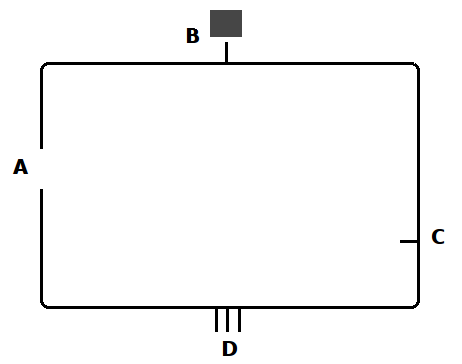
\includegraphics[]{figur.png}
\endcenter
\caption{Exempelbana. Punkt A i figuren visar en upplockningsstation, B ett stopp, C ett avbrott och D en avlämningsstation.}
\end{figure}